\documentclass[../Notes.tex]{subfiles}

\usepackage{tikz}

\begin{document}
    \subsection*{Motion in One Direction}

    \begin{center}
        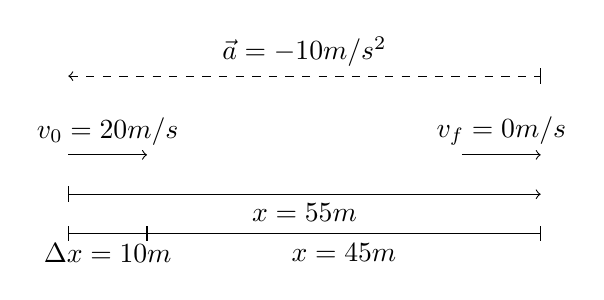
\begin{tikzpicture}
            \draw[->] (0, 0.5) -- (1, 0.5) node [midway, above]{$v_0 = 20 m/s$};
            \draw[->] (5, 0.5) -- (6, 0.5) node [midway, above]{$v_f = 0 m/s$};
            \draw[|->] (0,0) -- (6,0) node[midway, below] {$x = 55m$};
            \draw[|-|] (0, -0.5) -- (1, -0.5) node[midway, below] {$\Delta x = 10m$};
            \draw[|-|] (1, -0.5) -- (6, -0.5) node[midway, below] {$x = 45m$};
            \draw[dashed, <-|] (0, 1.5) -- (6,1.5) node[midway, above] {$\vec{a} = -10m/s^2$};
        \end{tikzpicture}
    \end{center}

    \subsection*{Motion on Incline}


\end{document}